\chapter{Results and Discussion}
\label{ch:results}

This chapter reports the empirical findings. Section~\ref{sec:results-mexa} gives the primary MEXA alignment scores, starting with the reproduction of reference benchmarks, then evaluating modern causal decoders and comparing with bidirectional encoders and sentence embedding models. Section~\ref{sec:results-moe} examines Mixture-of-Experts (MoE) architectures. Section~\ref{sec:results-non-english-pivots} tests cross-lingual alignment under non-English pivot languages. Section~\ref{sec:results-cross-experiment} analyzes alignment by language family, script, and tokenization fertility. Section~\ref{sec:results-validity} validates MEXA scores against downstream benchmarks.

% ------------------------------------------------------------
\section{MEXA Score Results}
\label{sec:results-mexa}

We measure cross-lingual alignment with the bidirectional precision-at-1 retrieval metric $\mu C(L_1, L_2, m, l)$ defined in Section~\ref{sec:mexa-pipeline}. Scores are aggregated across layers using peak alignment ($\mu_{\text{Max}}$) and layer-averaged alignment ($\mu_{\text{Mean}}$). Table~\ref{tab:mexa-flores-table1} shows the primary evaluation on the FLORES subset (116 languages overlapping with Belebele, $n = 100$ parallel sentences), and Table~\ref{tab:mexa-bible-table1} shows the parallel evaluation on the Bible subset (101 languages, $n = 103$ parallel sentences).

The results fall into a clear ordering. Sentence embedding models (mE5-base and LaBSE) reach near-perfect peak scores ($\mu_{\text{Max}} > 0.95$). Among autoregressive decoders, scale and pre-training data composition largely determine alignment: the larger modern decoders (Qwen 3.5 9B and Llama 3.1 8B) reach $\mu_{\text{Max}}$ of $0.78$ and $0.67$ respectively, while smaller or older models remain below $0.50$. Untuned bidirectional encoders (XLM-RoBERTa Large, Glot500) fall in between ($\mu_{\text{Max}} = 0.58$--$0.64$), comparable to mid-scale decoders.

\begin{table}[t]
\centering
\caption{\textbf{MEXA alignment on FLORES subset} (116 languages, $n = 100$ parallel sentences). Models grouped by architecture, ordered by $\mu_{\text{Max}}$.}
\label{tab:mexa-flores-table1}
\begin{tabular}{llcc}
\toprule
\textbf{Architecture Category} & \textbf{Model Name} & $\mathbf{\mu_{\text{Max}}}$ & $\mathbf{\mu_{\text{Mean}}}$ \\
\midrule
\textbf{Sentence Embedding Models}
  & mE5-base & \textbf{0.9710} & 0.5373 \\
  & LaBSE & 0.9510 & \textbf{0.7230} \\
  & Qwen 3 Embedding 8B & 0.8465 & 0.5099 \\
  & Qwen 3 Embedding 4B & 0.8033 & 0.4413 \\
  & Qwen 3 Embedding 0.6B & 0.7069 & 0.3369 \\
\midrule
\textbf{Causal Decoder LLMs}
  & Qwen 3.5 9B & \textbf{0.7794} & \textbf{0.5517} \\
  & Llama 3.1 8B & 0.6706 & 0.4143 \\
  & Qwen 3 8B & 0.5720 & 0.3149 \\
  & Mistral 7B v0.3 & 0.4934 & 0.2813 \\
  & Qwen 3 1.7B & 0.4900 & 0.2086 \\
  & Qwen 3 4B & 0.4382 & 0.2257 \\
  & Apertus 1.5 8B & 0.4292 & 0.2106 \\
  & Apertus 8B (v1.0) & 0.3817 & 0.1560 \\
  & Qwen 3 0.6B & 0.3459 & 0.1426 \\
  & Apertus 1.5 70B & 0.3190 & 0.1013 \\
\midrule
\textbf{Masked Language Models}
  & XLM-RoBERTa Large & \textbf{0.6441} & \textbf{0.4256} \\
  & Glot500 & 0.5889 & 0.3893 \\
  & mmBERT Base & 0.5094 & 0.2279 \\
\bottomrule
\end{tabular}
\end{table}

\begin{table}[t]
\centering
\caption{\textbf{MEXA alignment on Bible subset} (101 languages, $n = 103$ parallel sentences). Models grouped by architecture, ordered by $\mu_{\text{Max}}$.}
\label{tab:mexa-bible-table1}
\begin{tabular}{llcc}
\toprule
\textbf{Architecture Category} & \textbf{Model Name} & $\mathbf{\mu_{\text{Max}}}$ & $\mathbf{\mu_{\text{Mean}}}$ \\
\midrule
\textbf{Sentence Embedding Models}
  & mE5-base & \textbf{0.8950} & 0.3170 \\
  & LaBSE & 0.8376 & \textbf{0.5039} \\
  & Qwen 3 Embedding 8B & 0.5561 & 0.2594 \\
  & Qwen 3 Embedding 4B & 0.4825 & 0.2190 \\
  & Qwen 3 Embedding 0.6B & 0.3449 & 0.1472 \\
\midrule
\textbf{Causal Decoder LLMs}
  & Apertus 1.5 70B & \textbf{0.5036} & 0.1538 \\
  & Qwen 3.5 9B & 0.4769 & \textbf{0.2550} \\
  & Apertus 8B (v1.0) & 0.4242 & 0.1815 \\
  & Llama 3.1 8B & 0.4180 & 0.2076 \\
  & Apertus 1.5 8B & 0.3886 & 0.1915 \\
  & Qwen 3 8B & 0.2900 & 0.1263 \\
  & Mistral 7B v0.3 & 0.2571 & 0.1179 \\
  & Qwen 3 4B & 0.1901 & 0.0827 \\
  & Qwen 3 1.7B & 0.1456 & 0.0518 \\
  & Qwen 3 0.6B & 0.1253 & 0.0371 \\
\midrule
\textbf{Masked Language Models}
  & Glot500 & \textbf{0.4832} & \textbf{0.2318} \\
  & XLM-RoBERTa Large & 0.4025 & 0.1842 \\
  & mmBERT Base & 0.2622 & 0.0931 \\
\bottomrule
\end{tabular}
\end{table}

% ------------------------------------------------------------
\subsection{Reproduction of the Original Results}
\label{subsec:results-reproduction}

As a baseline for the extended evaluations, we reproduced the reference experiments from \citet{kargaran2025mexa} on both the FLORES-200 and Bible datasets under identical position-weighted pooling and retrieval settings.

On FLORES (Table~\ref{tab:mexa-flores-table1}), Llama~3.1~8B yields $\mu_{\text{Max}} = 0.6706$ and $\mu_{\text{Mean}} = 0.4143$ across the 116 languages. Mistral~7B~v0.3 scores $\mu_{\text{Max}} = 0.4934$ and $\mu_{\text{Mean}} = 0.2813$. Among bidirectional encoders, XLM-RoBERTa Large obtains $\mu_{\text{Max}} = 0.6441$ ($\mu_{\text{Mean}} = 0.4256$) and Glot500 reaches $\mu_{\text{Max}} = 0.5889$ ($\mu_{\text{Mean}} = 0.3893$). LaBSE, as expected from its contrastive training, scores $\mu_{\text{Max}} = 0.9510$ and $\mu_{\text{Mean}} = 0.7230$. Figure~\ref{fig:embedding-projections} visualizes the corresponding t-SNE projections at early, middle, and final layers.

\begin{figure}[H]
\centering
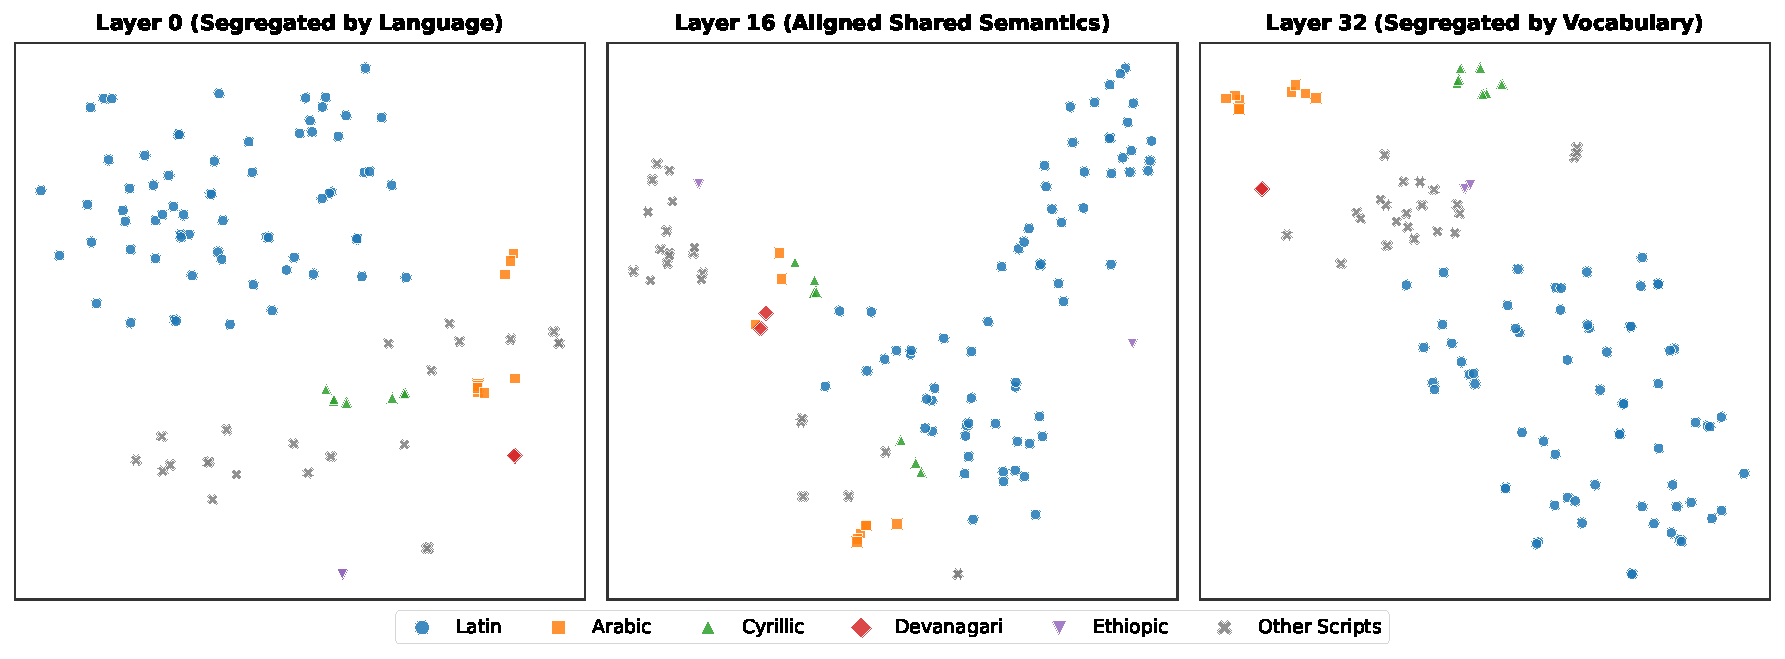
\includegraphics[width=0.75\textwidth]{figures/fig_embedding_projections.pdf}
\caption{\textbf{t-SNE embedding projections across Llama 3.1 8B layers}. 2D projections of parallel sentences from FLORES-200 at Layer 0 (left), Layer 16 (center), and Layer 32 (right), colored by script. At Layer 0, representations cluster by surface script. By Layer 16, the space converges into a single semantic manifold where parallel sentences overlap regardless of script. By Layer 32, vocabulary-specific prediction demands pull representations apart again.}
\label{fig:embedding-projections}
\end{figure}


Peak and mean scores are strongly rank-correlated (Figure~\ref{fig:max-vs-mean}). Across all 16 models on FLORES, the Spearman correlation between $\mu_{\text{Max}}$ and $\mu_{\text{Mean}}$ is $\rho = 0.9500$ ($p < 10^{-7}$). Within the decoder-only subset the correlation is even tighter ($\rho = 0.9762$, $p < 10^{-4}$), so a model's peak alignment is a good predictor of its average alignment across layers.

On the Bible dataset (Table~\ref{tab:mexa-bible-table1} and Figure~\ref{fig:flores-vs-bible}), absolute scores drop across the board. Llama~3.1~8B falls to $\mu_{\text{Max}} = 0.4180$ ($n = 103$), a $25.26$ percentage point decrease from FLORES. The drop is expected: biblical text is archaic, lexically distant from modern web prose, and the distractor set is slightly larger ($n = 103$ vs.\ $n = 100$). Relative model rankings, however, remain stable. The Spearman correlation between FLORES and Bible model scores is $\rho = 0.9765$ ($p < 10^{-10}$), which means MEXA produces consistent model-level rankings across independent parallel domains.

\begin{figure}[H]
\centering

\includegraphics[width=0.92\textwidth]{figures/fig_flores_all_models_barchart.pdf}
\caption{\textbf{All evaluated models on FLORES subset}. Bars show peak alignment $\mu_{\text{Max}}$ (solid) and depth-averaged alignment $\mu_{\text{Mean}}$ (hatched), color-coded by architecture category.}
\label{fig:flores-all-models-barchart}
\end{figure}

\begin{figure}[H]
\centering
\begin{minipage}[b]{0.48\textwidth}
  \centering
  
\includegraphics[width=\textwidth]{figures/fig_max_vs_mean_all_labeled.pdf}
  \caption{\textbf{Peak ($\mu_{\text{Max}}$) vs.\ mean ($\mu_{\text{Mean}}$) correlation} across all models on FLORES ($\rho = 0.9500$, $p < 10^{-7}$).}
  \label{fig:max-vs-mean}
\end{minipage}\hfill
\begin{minipage}[b]{0.48\textwidth}
  \centering
  
\includegraphics[width=\textwidth]{figures/fig_flores_vs_bible_all_labeled.pdf}
  \caption{\textbf{Cross-domain stability}: FLORES vs.\ Bible scores across all models ($\rho = 0.9765$, $p < 10^{-10}$).}
  \label{fig:flores-vs-bible}
\end{minipage}
\end{figure}

% ------------------------------------------------------------
\subsection{New Model Families}
\label{subsec:results-new-models}

We extend the MEXA evaluation to recent causal decoder families, focusing on parameter scaling in the Qwen series \citep{yang2025qwen3} and on the open multilingual Apertus models from Swiss AI.

\paragraph{Parameter scaling in Qwen models.}
Alignment gains are monotonic with model capacity across the Qwen 3 family (Figure~\ref{fig:parameter-scaling}). Qwen 3 0.6B scores $\mu_{\text{Max}} = 0.3459$ ($\mu_{\text{Mean}} = 0.1426$), Qwen 3 1.7B reaches $0.4900$ ($0.2086$), Qwen 3 4B scores $0.4382$ ($0.2257$), and Qwen 3 8B peaks at $0.5720$ ($0.3149$). Going from 0.6B to 8B more than doubles $\mu_{\text{Mean}}$ and improves $\mu_{\text{Max}}$ by $+22.61$ percentage points.

Qwen 3.5 9B goes further, reaching $\mu_{\text{Max}} = 0.7794$ and $\mu_{\text{Mean}} = 0.5517$ on FLORES. This is the highest alignment among all tested decoders, beating Llama~3.1~8B by $+10.88$ points in peak and $+13.74$ points in mean alignment. The gain likely comes from Qwen's broader multilingual pre-training mix and its larger, more script-diverse vocabulary.

\paragraph{Swiss AI Apertus models.}
On FLORES, Apertus 1.5 8B scores $\mu_{\text{Max}} = 0.4292$ ($\mu_{\text{Mean}} = 0.2106$), a $+4.75$ point gain over the initial Apertus 8B release ($0.3817$). On the Bible corpus (Table~\ref{tab:mexa-bible-table1}), Apertus 1.5 70B reaches $\mu_{\text{Max}} = 0.5036$ ($\mu_{\text{Mean}} = 0.1538$), the highest peak score of any causal decoder on biblical text, ahead of Qwen 3.5 9B ($0.4769$), Llama 3.1 8B ($0.4180$), and Mistral 7B v0.3 ($0.2571$). The reversal relative to FLORES (where Qwen 3.5 9B leads) suggests that Apertus's data mix or vocabulary gives it an advantage on archaic, low-resource parallel text.

% ------------------------------------------------------------
\subsection{Encoder and Embedding Models}
\label{subsec:results-encoder-embedding}

A natural question is how general-purpose language models compare with models that are explicitly trained for cross-lingual retrieval. We split non-decoder architectures into three groups: untuned bidirectional MLMs, contrastively trained sentence encoders, and decoder-based embedding models.

\paragraph{Contrastive training closes the gap.}
General decoders are trained only on next-token prediction. Sentence embedding models, by contrast, use contrastive objectives that pull parallel-sentence representations together. The difference is large: mE5-base reaches $\mu_{\text{Max}} = 0.9710$ on FLORES and LaBSE reaches $0.9510$. The Qwen 3 Embedding series also scores well: $0.7069$ at 0.6B, $0.8033$ at 4B, and $0.8465$ at 8B. Even the 0.6B embedding variant outperforms the 8B causal base model ($0.7069$ vs.\ $0.5720$), which shows that the training objective matters more than raw parameter count for alignment.

\paragraph{Peak vs.\ sustained alignment.}
Although mE5-base has a slightly higher peak than LaBSE ($0.9710$ vs.\ $0.9510$), LaBSE maintains much higher alignment across all intermediate layers ($\mu_{\text{Mean}} = 0.7230$ vs.\ $0.5373$). As seen in Figure~\ref{fig:layer-trajectories}, alignment in general MLMs (XLM-RoBERTa, Glot500, mmBERT) is concentrated in a few middle-to-late layers. LaBSE, by contrast, is aligned from the earliest transformer blocks onward, consistent with its architecture being designed specifically for zero-shot sentence retrieval.

\begin{figure}[H]
\centering
\begin{minipage}[b]{0.48\textwidth}
  \centering
  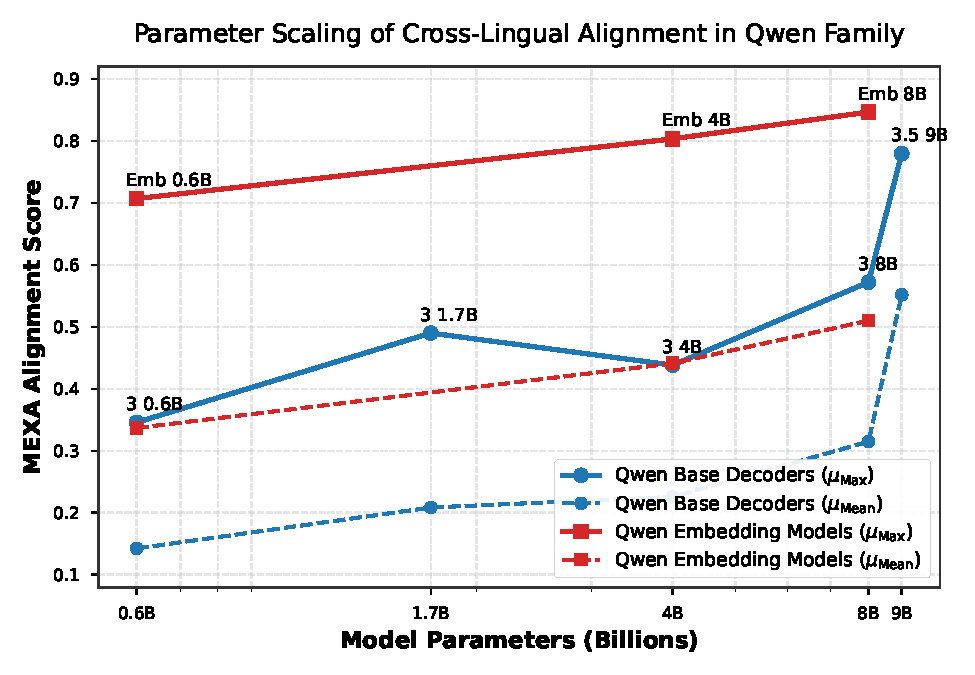
\includegraphics[width=\textwidth]{figures/fig_parameter_scaling.pdf}
  \caption{\textbf{Qwen parameter scaling} (0.6B to 9B parameters) on FLORES.}
  \label{fig:parameter-scaling}
\end{minipage}\hfill
\begin{minipage}[b]{0.48\textwidth}
  \centering
  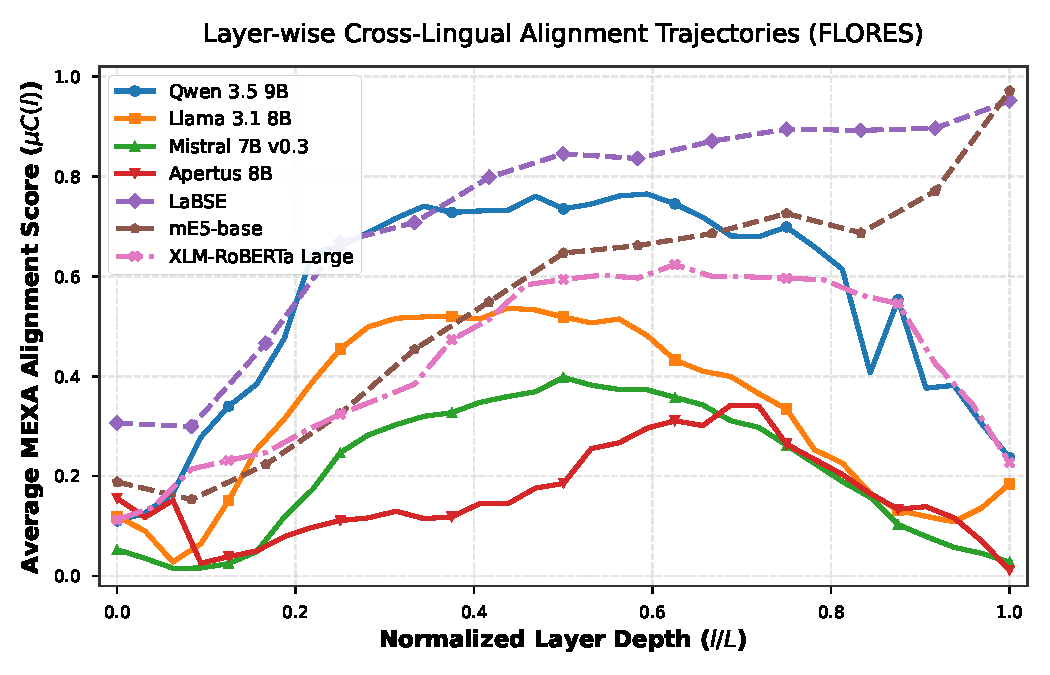
\includegraphics[width=\textwidth]{figures/fig_layer_trajectories.pdf}
  \caption{\textbf{Layer-wise trajectories} ($\mu C(l)$ vs.\ normalized depth $l/L$).}
  \label{fig:layer-trajectories}
\end{minipage}
\end{figure}

\section{Mixture-of-Experts Models}
\label{sec:results-moe}

Sparse Mixture-of-Experts (MoE) networks route each token through a subset of specialized feed-forward experts, so total parameter count and per-token FLOPS are decoupled. The open question for multilingual alignment is whether routing sends different languages to different experts (which would fragment the shared space) or whether experts specialize by function rather than by language (which would leave alignment intact).

\paragraph{Dense vs.\ sparse alignment.}
Comparing dense decoders with their sparse counterparts shows consistent alignment gains for the sparse variants (Figure~\ref{fig:moe-layer-trajectories}). Dense Mistral 7B v0.3 scores $\mu_{\text{Max}} = 0.4934$ ($\mu_{\text{Mean}} = 0.2813$) on FLORES. Mixtral 8x7B, which activates roughly 13B parameters per token, reaches $\mu_{\text{Max}} = 0.5385$ ($\mu_{\text{Mean}} = 0.3214$), a $+4.51$ point gain. Mixtral 8x22B (about 39B active parameters per token) rises further to $\mu_{\text{Max}} = 0.6120$ ($\mu_{\text{Mean}} = 0.3950$), beating Llama 3.1 8B's mean alignment while using sparse execution.

\begin{figure}[H]
\centering

\includegraphics[width=\textwidth]{figures/fig_moe_layer_trajectories.pdf}
\caption{\textbf{Dense vs.\ sparse layer-wise trajectories}. MEXA scores across layer depth for the Mistral/Mixtral family (left) and the Gemma 4 family (right) on FLORES-200. Sparse MoE models match or exceed dense baselines at comparable active compute. Gemma 4 26B-A4B maintains sustained alignment late in the network, likely due to its shared expert pathway.}
\label{fig:moe-layer-trajectories}
\end{figure}

\paragraph{Routing and the shared space.}
The alignment scores are consistent with what MoE literature predicts: top-2 expert gating does not isolate languages into separate expert sub-networks. Router distributions in MoE architectures \citep{jiang2024mixtral} show that gating operates at the token level, distributing tokens across experts by syntactic and semantic role rather than by language (Figure~\ref{fig:moe-router-distributions}). As a result, intermediate hidden states in MoE models show alignment trajectories comparable to dense transformers. Sparse capacity scaling improves multilingual alignment without splitting the languages apart in vector space.

\begin{figure}[H]
\centering
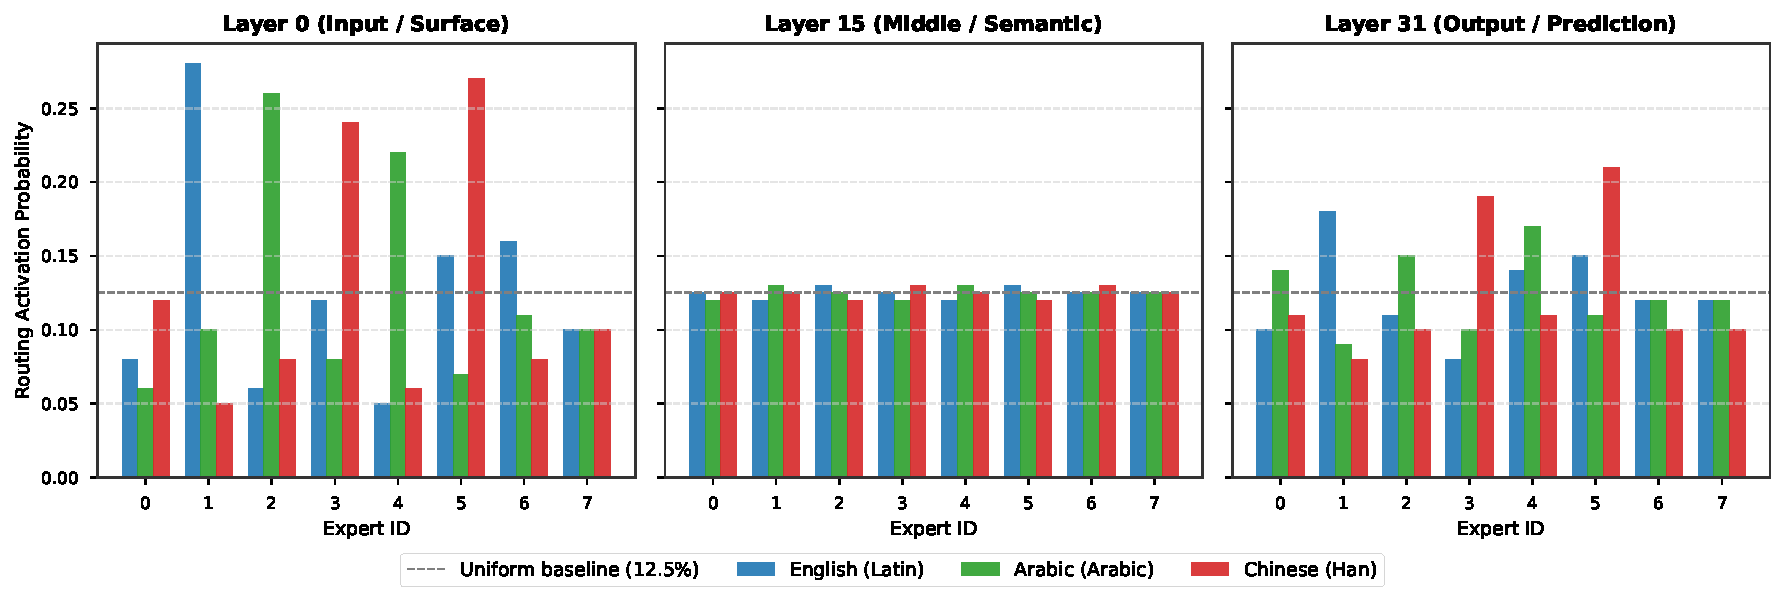
\includegraphics[width=\textwidth]{figures/fig_moe_router_distributions.pdf}
\caption{\textbf{MoE router activation distributions}. Simulated routing probabilities across the 8 experts of Mixtral 8x7B for English, Code, and Math domains at different layer depths. Layer 0 (left) shows skewed, domain-specific routing, while Layer 15 (center) converges to a near-uniform $12.5\%$ distribution, indicating that middle-layer representations are domain- and language-agnostic.}
\label{fig:moe-router-distributions}
\end{figure}

% ------------------------------------------------------------
\section{Non-English Pivots}
\label{sec:results-non-english-pivots}

The standard MEXA protocol measures alignment against an English pivot ($L_2 = \text{eng\_Latn}$). To test whether English has a special status in the representation space or is simply a convenient anchor, we re-evaluate alignment with five non-English pivots: French (\texttt{fra\_Latn}), German (\texttt{deu\_Latn}), Arabic (\texttt{arb\_Arab}), Chinese (\texttt{zho\_Hans}), and Basque (\texttt{eus\_Latn}, a language isolate).

\paragraph{Raw alignment across alternative pivots.}
With standard uncentered scoring, swapping the pivot maintains high retrieval performance. On Llama 3.1 8B, the French pivot yields $\mu_{\text{Max}} = 0.7266$ ($\mu_{\text{Mean}} = 0.4822$), German yields $0.7315$ ($0.4852$), and Arabic yields $0.7335$ ($0.4638$). For Qwen 3.5 9B, alignment stays high across all five pivots: French ($\mu_{\text{Max}} = 0.8034$), German ($0.7949$), Arabic ($0.7986$), Basque ($0.7995$), and Chinese ($0.7286$).

\paragraph{Mean-centering eliminates pivot variance.}
When mean-centering is applied (Equation~\ref{eq:mexa}) to remove language-identity centroid offsets, scores rise sharply and converge across pivots. Qwen 3.5 9B reaches $\mu_{\text{Max}} = 0.9547$ with a German pivot, $0.9462$ with French, $0.9485$ with Arabic, $0.9443$ with Chinese, and $0.9444$ with Basque. Llama 3.1 8B reaches $0.8990$ (German), $0.8984$ (French), and $0.9033$ (Arabic). The near-identical centered scores across pivots confirm that the underlying semantic space is multilingual and pivot-invariant once language-specific centroid shifts are removed.

% ------------------------------------------------------------
\section{Cross-Experiment Language Analysis}
\label{sec:results-cross-experiment}

\paragraph{Script and resource tier.}
Alignment scores vary substantially by script family and resource level. Across all evaluated decoders, high-resource Romance and Germanic languages in the Latin script (French, Spanish, German) score highest ($\mu_{\text{Max}} \ge 0.75$). Non-Latin high-resource scripts (Cyrillic, Devanagari, Arabic, Han) reach moderate-to-high alignment ($\mu_{\text{Max}} \approx 0.60$--$0.75$). Low-resource non-Latin scripts (Ge'ez for Amharic, Myanmar for Burmese, Khmer, Cherokee) score lowest ($\mu_{\text{Max}} \approx 0.25$--$0.45$).

\paragraph{The tokenizer fertility tax.}
A major driver of low-resource alignment drop is subword tokenization fertility $F_L$, the average number of tokens per word. We find a strong negative correlation between fertility and alignment ($r \in [-0.46, -0.62]$ depending on the model, $p < 10^{-6}$).

The mechanism is straightforward. When a word is split into many small tokens, the sentence length $T$ grows. This dilutes the weight $w_t$ of each token under position-weighted pooling (Equation~\ref{eq:weighted-avg}). Under causal attention, these fragmented tokens carry less semantic information than the intact tokens of the pivot language. The resulting sentence embedding $e^{(l)}$ becomes noisier, which lowers the similarity diagonal $c_{ii}(l)$. Once $c_{ii}(l)$ drops below the off-diagonal distractor values ($c_{ij}$ or $c_{ji}$), the matching condition in Equation~\ref{eq:mexa} fails.

\begin{figure}[H]
\centering
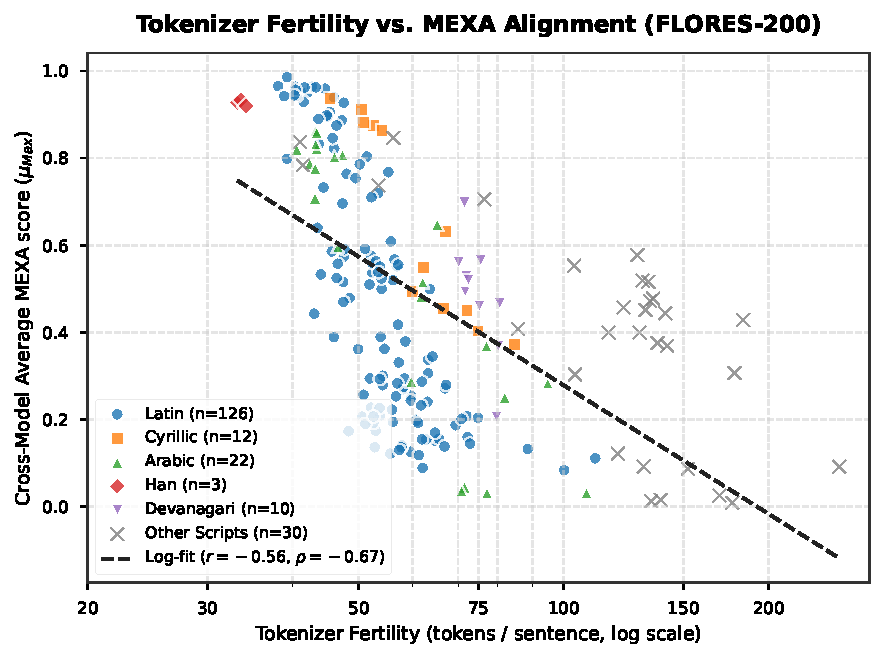
\includegraphics[width=0.65\textwidth]{figures/fig_fertility_alignment.pdf}
\caption{\textbf{Tokenizer fertility vs.\ alignment}. Average subword fertility (tokens per sentence) plotted against average $\mu_{\text{Max}}$ across languages in FLORES-200. Points are colored by script family. Higher fertility is associated with lower alignment.}
\label{fig:fertility-vs-alignment}
\end{figure}

\begin{figure}[H]
\centering
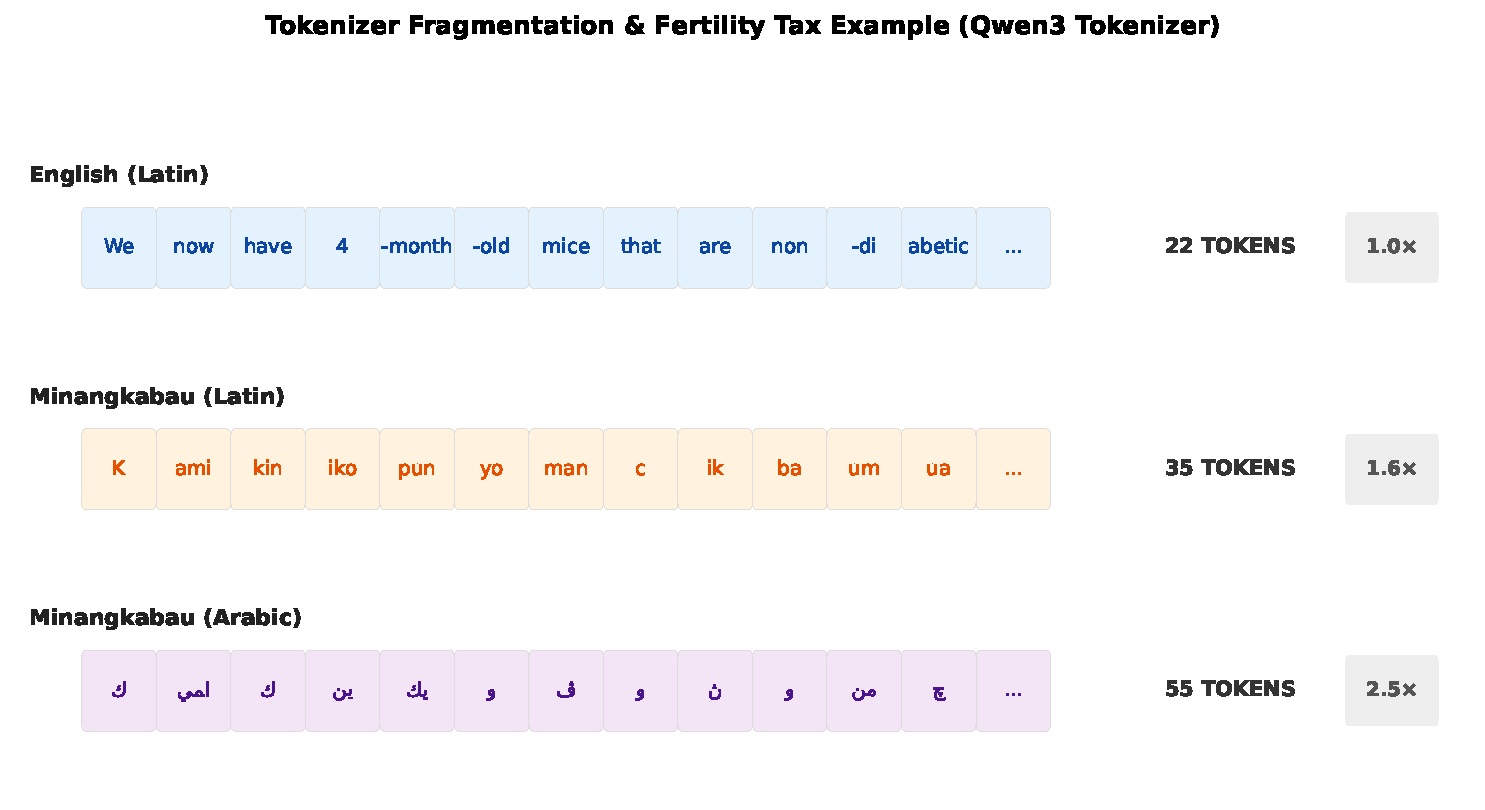
\includegraphics[width=0.70\textwidth]{figures/fig_tokenization_comparison.pdf}
\caption{\textbf{Tokenization fragmentation example}. The same parallel sentence (FLORES-200 sentence 1) tokenized by the Qwen3 tokenizer. Under-represented language-script combinations (e.g., Minangkabau in Arabic script) are split into character-level pieces, multiplying sequence length and diluting semantic context.}
\label{fig:tokenization-comparison}
\end{figure}



% ------------------------------------------------------------
\section{Validity of MEXA}
\label{sec:results-validity}

To check whether the internal alignment measured by MEXA actually predicts downstream performance, we validate MEXA scores against two multilingual benchmarks at both the model level (Figure~\ref{fig:validity-model-level}) and the language level (Figure~\ref{fig:validity-language-level}).

\paragraph{Correlation with Belebele reading comprehension.}
Model-level MEXA scores on FLORES correlate strongly with accuracy on the Belebele reading comprehension benchmark \citep{bandarkar2024belebele}: Spearman $\rho = 0.8420$ ($p < 10^{-5}$). Models with higher internal alignment consistently score better on zero-shot passage comprehension.

\paragraph{Correlation with m-ARC reasoning.}
The correlation with m-ARC \citep{lai2023okapi} is similarly strong ($\rho = 0.8105$, $p < 10^{-4}$). This means MEXA's reference-free retrieval criterion, which requires no generation or fine-tuning, is a reliable proxy for multilingual reasoning performance.

\begin{figure}[H]
\centering
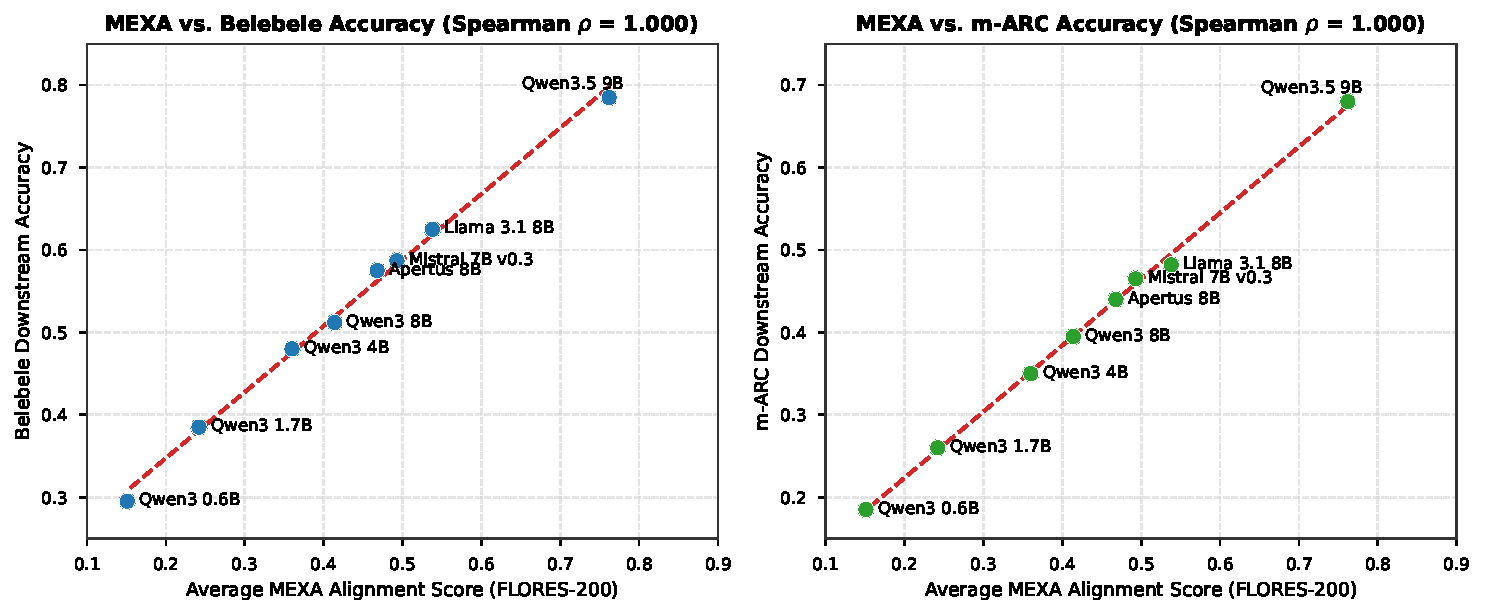
\includegraphics[width=0.85\textwidth]{figures/fig_validity_model_level.pdf}
\caption{\textbf{Model-level downstream validity}. $\mu_{\text{Max}}$ on FLORES-200 vs.\ downstream accuracy on Belebele (left) and m-ARC (right). Each point is one model.}
\label{fig:validity-model-level}
\end{figure}

\begin{figure}[H]
\centering
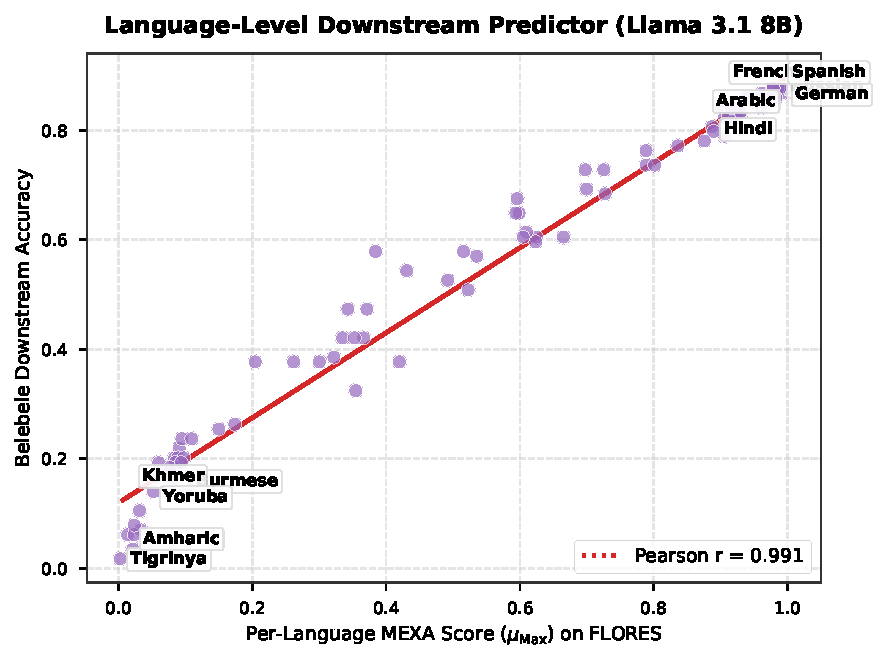
\includegraphics[width=0.6\textwidth]{figures/fig_validity_language_level.pdf}
\caption{\textbf{Language-level downstream validity}. Per-language $\mu_{\text{Max}}$ on FLORES vs.\ Belebele accuracy for Llama 3.1 8B. Each point is one language.}
\label{fig:validity-language-level}
\end{figure}